\chapter{Spektrale Methoden\label{chapter:klima}}
\lhead{Spektrale Methoden}
\begin{refsection}
\chapterauthor{Peter Nötzli}



\section{Einleitung
\label{klima:einleitung}}
\rhead{Einleitung}

\begin{figure}
\centering
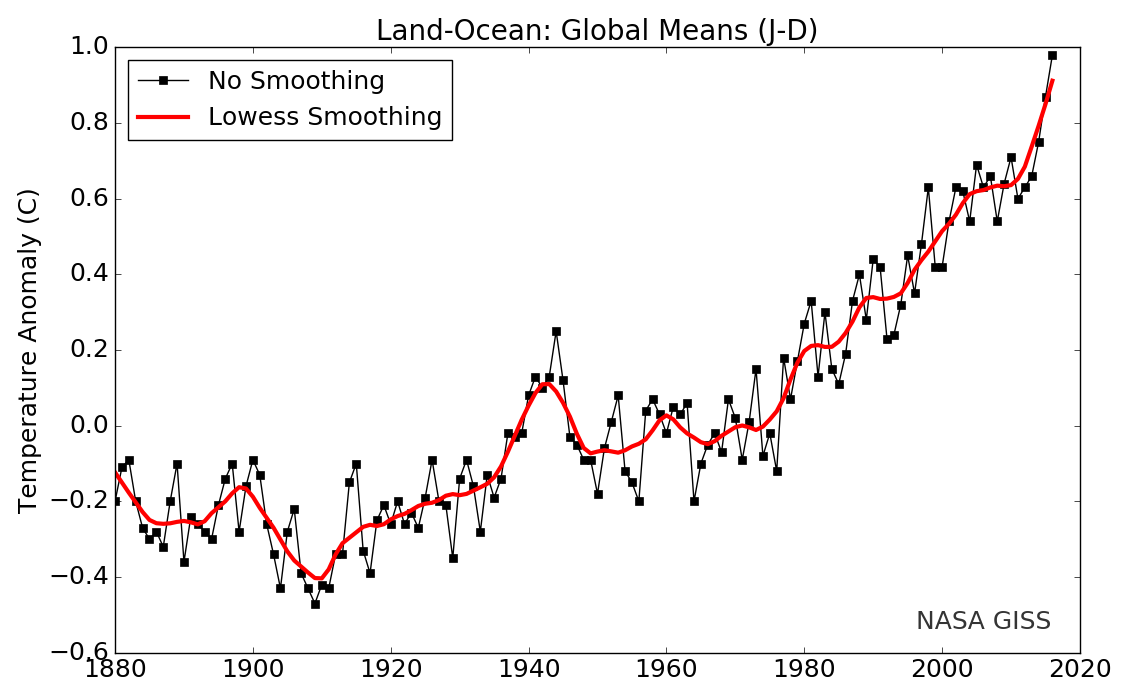
\includegraphics[width=\hsize]{klima/nasa_giss.png}
\caption{Grafik der globalen Jahresmitteltemperaturen seit 1880. Quelle: National Aeronautics and Space Administration Goddard Institute for Space Studies kurz NASA GISS \url{https://data.giss.nasa.gov/gistemp/graphs/customize.html}.
\label{klima:einleitung:nasa}}
\end{figure}

Die Klimaerwärmung schreitet voran, gleichzeitig, oder gerade deswegen kommen in der Gesellschaft dazu immer mehr Fragen auf. Gibt es eine Klimaerwärmung? Wie entwickelt sich diese? Was bedeutet dies für uns? Betrifft es mich überhaupt? Die erste und wohl einfachste Frage vorweg, ja es gibt die Klimaerwärmung. Dies ist deutlich zu erkennnen wenn wir die globale Temperaturentwicklung seit 1880 bis heute betrachten (Abbildung~\ref{klima:einleitung:nasa}). Diese Frage ist deshalb einfach zu beantworten, da diese nach einer Entwicklung frägt welche bereits, oder zumindest teilweise, in der Vergangeheit liegt. Die Auswirkungen dieser Entwicklung und wie weit diese noch fortschreitten wird sind Dinge, welche in der Zukunft liegen. Somit kann für die restlichen Fragen und auch viele der nicht gestellten Fragen keine pauschale Antwort gegeben werden. Obwohl eine Tendenz der Temperaturentwicklung erkennbar ist, diese mit ein bisschen Gefühl weiter zu führen und abzuschätzen kann wohl nicht richtig sein, da es sämtliche Faktoren welche einen Einfluss auf das Klima haben ignoriert. Da wir dennoch gerne wissen wollen welche Einflüsse welche Auswirkungen haben und wir auch nicht warten möchtenx bis es bereits zu spät ist, müssen wir auf Klimamodelle zurückgreifen. Wie so ein Klimamodell ausschauen könnte und wie es aufgebaut sein kann soll in diesem Kapitel aufgezeigt werden.



\section{Geschichte der Numerischen Strömungsmechanik
\label{section:klima:geschichte}}
\rhead{Geschichte}
Die numerische Strömungsmechanik, heute auch als CFD bekannt (Computational Fluid Dynamics) bezeichnet eine etablierte Methode, um verschiedenste Problemstellungen der Strömungsmechanik approximativ mit numerischen Modellen zu lösen. Die Validierung der Methoden erfolgt durch den Vergleich mit quantitativen Experimenten.



\subsection{Entstehung der Wettervorhersagen
\label{subsection:klima:wetter}}
Am Anfgang war das Wetter. Dann kam der Mensch und wollte wissen, wie das Wetter in Zukunft sein wird. Dies aus verschiedensten Gründen so wollen wir heute gerne wissen, welches Wetter am Wochenende ist, damit wir bereits anfangs Woche einen Ausflug organisieren können.

Bedeutung hatten Wettervorhersagen, früher wie heute, so kann eine Wettervorhersage wesentlichen Einfluss auf das Ernteglück haben. So entstanden schon früh sogenannte Bauernregeln, diese gingen meist davon aus dass sich das Wetter aufgrund Wetterereignissen an bestimmten Tagen in eine gewisse Richtung entwickeln. Die Korrektheit solcher Aussagen sind wohl eher Zufälle als korrekte Vorhersagen, so sind es eher die ähnlichen Wetterverhältnisse der jeweiligen Jahreszeit welche solch eine Regel von Zeit zu Zeit als korrekt erscheinen lässt. Jedoch waren verschiedenste Naturphänomene bereits bekannt, als Beispiel die Silberdiestel, auch als Wetterdiestel bekannt, welche seine Blütenblätter bei erhöhter Luftfeuchtigkeit aufrollt und so vor nahendem Regen warnen kann.1660 erkannte Otto von Guericke erstmals den Zusammenhang zwischen abfallendem Luftdruck und dem Aufziehen eines Unwetters.

Anfangs des 19. Jahrhunderts entstanden in Europa die ersten Wetterstationen, es waren jedoch noch keine Wettervorhersagen möglich. Dies aus dem einfachen Grund, da sich das Wetter schneller in eine nahende Stadt bewegen konnte als man die Daten dort hinbringen hätte können.

1835 konnte mit dem aufkommen der Telegrafie dieses Problem gelöst werden, erstmals waren einfache Prognosen möglich. Diese reichten oft nur einzelne Tage in die Zukunft und waren lokal begrenzt. Die Genauigkeit dieser ist nicht mit heutigen Massstäben vergleichbar.

Vilhelm Bjerknes (1862-1951) war der erste, welcher erkannte dass die Problemstellung der Wettervorhesage sich aus Physik und Mathematik zusammensetzt. Im wesentlichen stellte er fest, dass für die Berechnung der Strömung der Atmosphäre genaue Kenntnisse der Grundgesetze und der Anfangsbestimmungen notwendig und ausreichend für eine Wettervorhersage sind.



\subsection{Lewis Fry Richardson
\label{subsection:klima:richardson}}

\begin{figure}
\centering
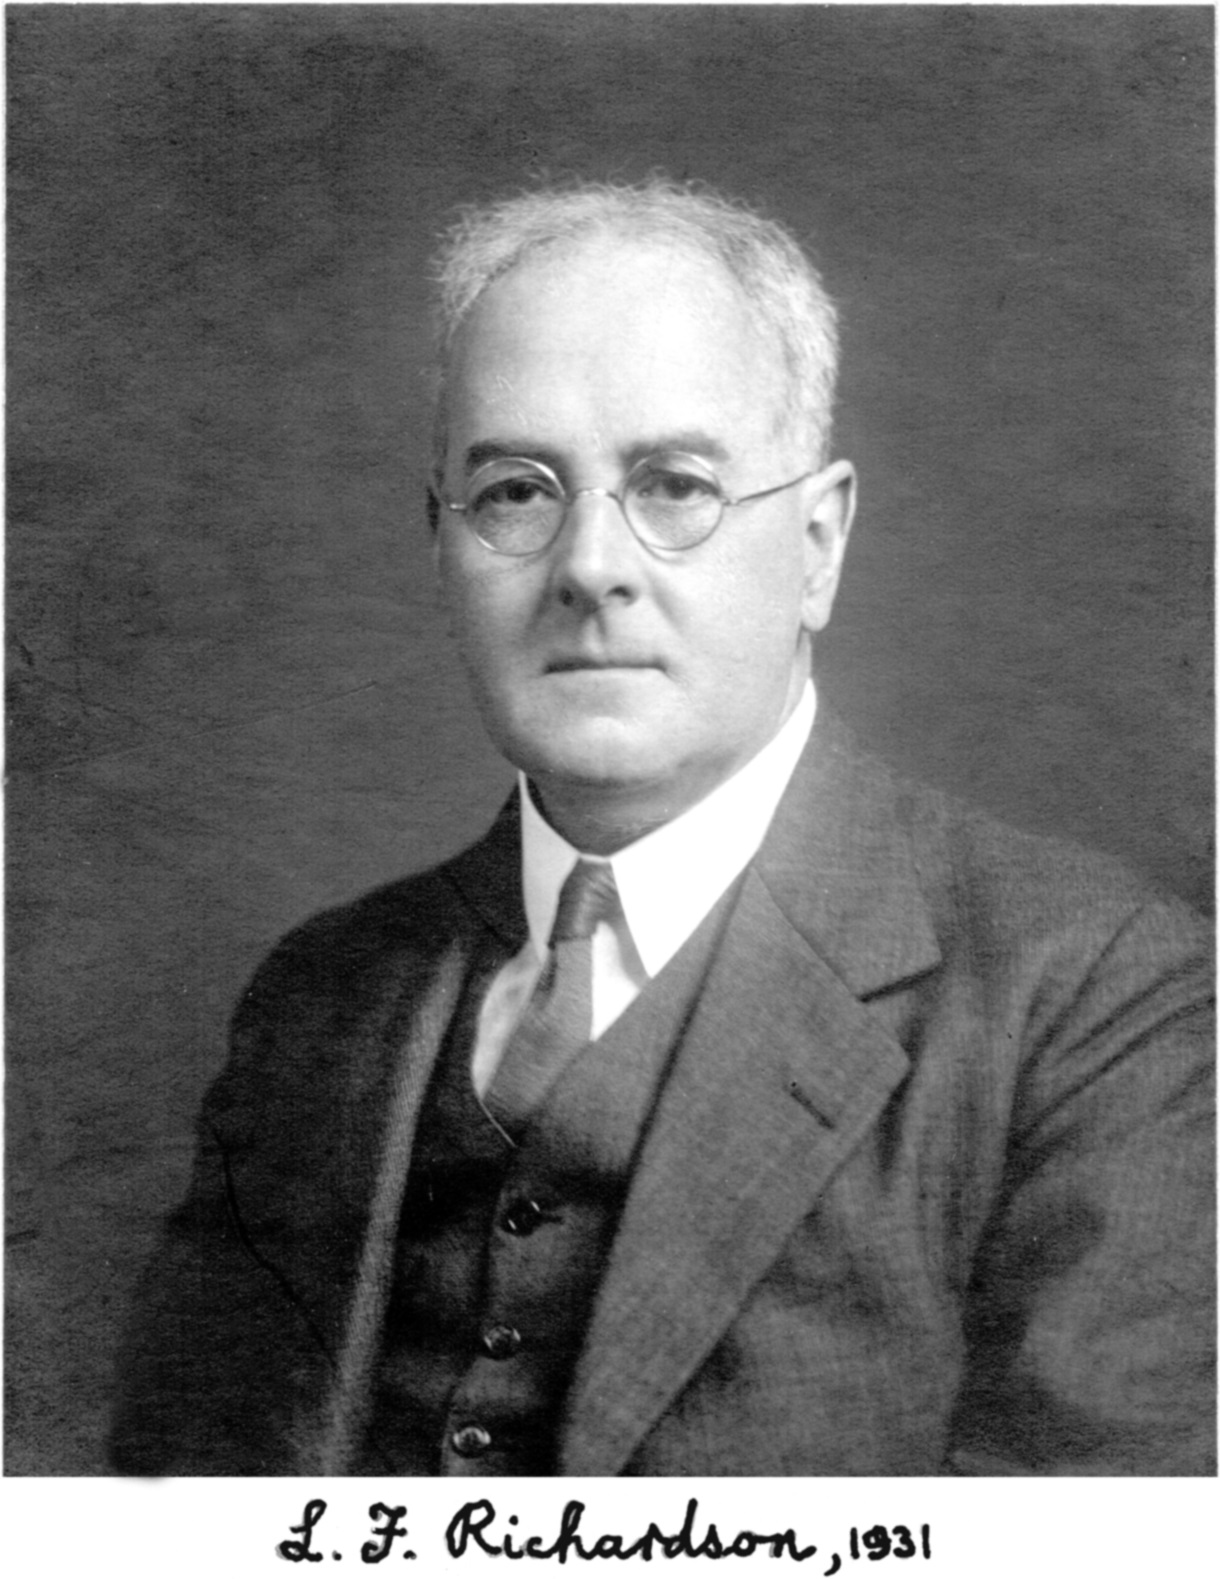
\includegraphics{klima/richardson.jpg}
\caption{Lewis Fry Richardson \cite{klima:biography}
\label{klima:geschichte:richardson}}
\end{figure}

Lewis Fry Richardson (1881-1953) Abbildung~\ref{klima:geschichte:richardson} veröffentlichte 1922 seine Arbeit mit dem Titel {\em Weather Prediction by Numerical Process}, in welcher er die erste numerische Wettervorhersage tätigte. Für seine Berechnungen, die er um 1917 durchführte, verwendete er Druck- und Temperatur-Daten verschiedenster Stationen in Europa. Er legte für seine Berechnung ein Gitter über Europa, dieses hatte eine Breite von 2°89' und eine Länge von 1°80', und 5 vertikale Layer. Dies entspricht in etwa einer Abmessung von 320km mal 200km je Feld und umfasst ingesamt etwa 150 Punkte an welchen die Drucktendenz berechnet werden sollte. Er verwendete dabei die horizontalen Impulserhaltungsgleichungen, die ideale Gasgleichung und die Kontinuitätsgleichung \eqref{skript:speziell:kontinuitaetsgleichung} (diese wurde auf Seite \pageref{skript:speziell:kontinuitaetsgleichung} bereits behandelt). Die Vorhersage für 24 Stunden bedeutete dabei einen Rechenaufwand von 3 Monaten. Im wesentlichen basierte die Berechnung auf einer Unterteilung in die einzelnen Zellen welche jeweils mit 7 Werten befüllt waren. Dies waren der Luftdruck, Temperatur, Dichte, Luftfeuchtigkeit und den Volumenströmen richtung Norden, Osten und Aufwärts.

Die erste Berechnung von Richardson lieferte dann auch ein Resultat, welches einen Druckabfall von 145mbar in 6h voraussagte. Eine solch grosse Veränderung ist absolut unrealistisch und nicht einmal im Zentrum eines Sturmtiefes möglich. Das Problem war, dass die Daten des Boden-Drucks, welche als Anfangsbedinungen verwendet wurden, Fehler enthielten. Diese Fehler führten dazu, dass sich während der numerischen Prozedur die Werte aufschaukelten und somit zu hohen Drucktendenzen führten. (Eine Berechnung aufgrund der selben Beobachtungsdaten, die jedoch zu Beginn gefiltert werden, führt mit Richardson's Algorithmus zu plausiblen Vorhersagen, 3.2 mbar in 6h \cite{klima:stocker}).

Dies zeigt exemplarisch wie heikel die Anfangsbedingungen von Wetter- und Klimamodellen sich auf das Ergebniss auswirken können. Jedoch hätten selbst die besten Initialisierungswerte zu einer Instabilität geführt und eine Resultat für grosse Vorhersagezeiten verunmöglicht. Erst durch die Verfügbarkeit erster Computer in den 40er Jahren wurde Richardsons Arbeit zur  Wettervorhersage praktikabel und wurde gegen Ende des 2. Weltkriegs als taktisches Mittel eingesetzt.

\begin{figure}
\centering
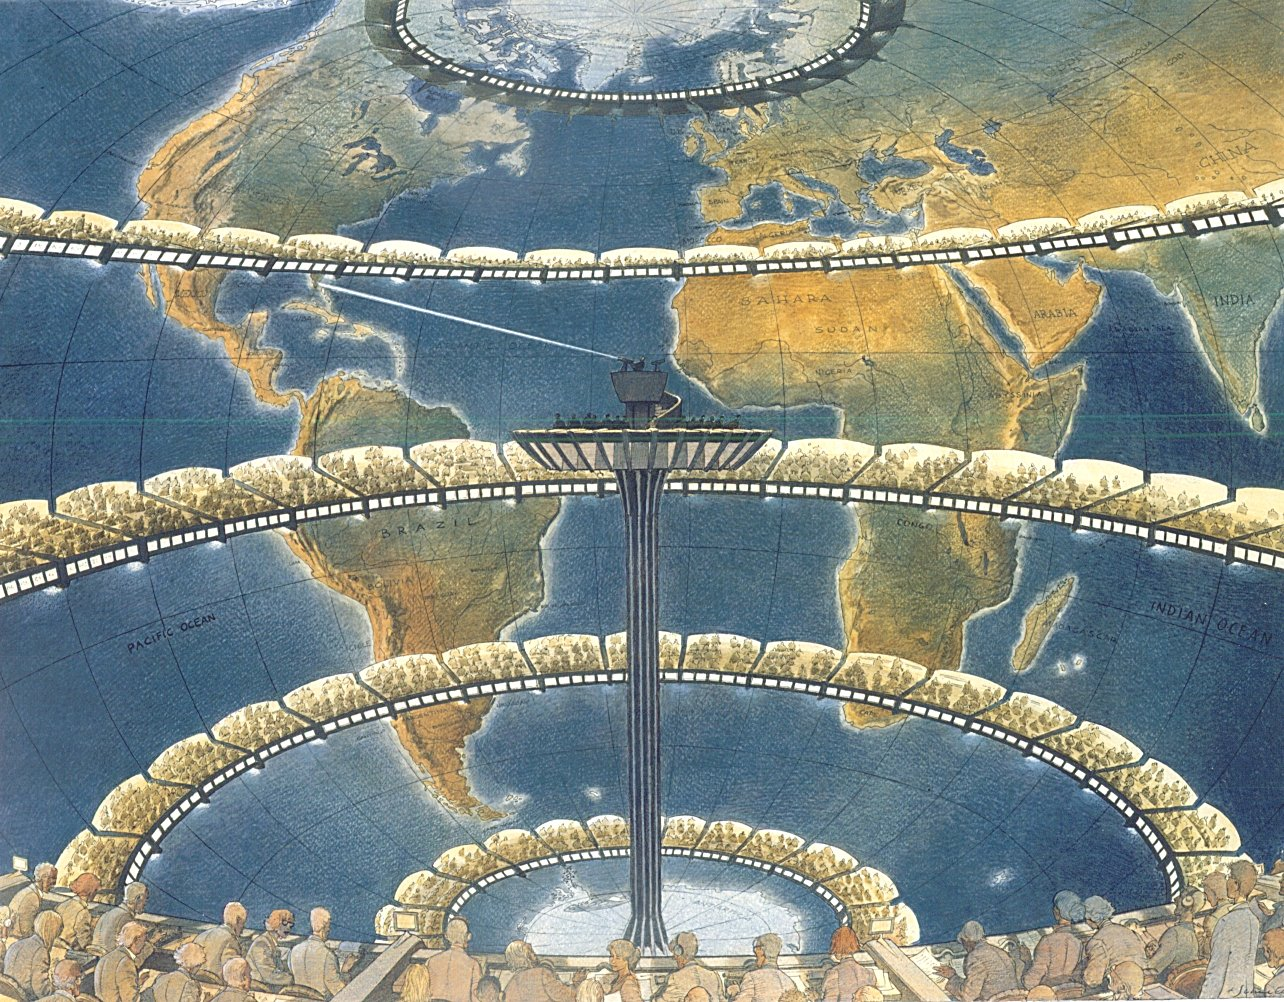
\includegraphics{klima/64000.jpg}
\caption{Interpretation eines Künstlers von Richardsons Vorhersage Fabrik \cite{klima:biography}
\label{klima:geschichte:richardson}}
\end{figure}

Richardson äusserte in seiner Arbeit die Idee einer Vorhersage Fabrik in welcher er mit 64'000 Rechnern (damit waren damals noch Menschen gemeint), welche gleichzeitig Berechnungen durchführten und zum weiterrechnen jeweils die Werte ihrer Nachbarzellen übernehmen sollten, das Wetter für den ganzen Planeten berechnen könnte. Diese Idee wurde vom Künstler François Schuiten in der Abbildung~\ref{klima:geschichte:richardson} versinnbildlicht.

Zudem äusserte Richardson einen weiteren Traum:
\begin{quote}
Perhaps some day in the dim future it will be possible to advance the computations faster than the weather advances....
\end{quote}
Von diesem wissen wir, dass es heute nicht nur möglich ist, sondern werden mit jeden neuen Wettervorhersage daran erinnert, dass dies an jedem Tag aufs neue geschieht.



\subsection{Wettervorhersagen in der Schweiz
\label{section:klima:wettervorhersagen}}
\rhead{Wettervorhersagen}

Insgesamt haben wir in der Schweiz 7 private Wetterdienst-Anbieter und den Bundesbetrieb MeteoSchweiz. In diesem Abschnitt wird mehrheitlich auf MeteoSchweiz und deren Methoden eingegangen, dies weil MetheoSchweiz ihre Methoden im Internet öffentlich einsehbar teilen.

MeteoSchweiz betreibt mit SwissMetNet ein eigenes automatisches Messnetz welches ca.160 Station umfässt. Diese liefern alle 10min aktuelle Werte an die zentrale Datenbank der MeteoSchweiz. An einer Standardstation werden kontinuierlich Temperatur, Luftfeuchtigkeit, Luftdruck, Sonneneinstrahlung, Niederschlagsmenge, Windrichtung und -geschwindigkeit erfasst. Doch diese Stationen würden alleine nicht ausreichen, so arbeitet MeteoSchweiz auch mit kantonalen Fachstellen und anderen Institutionen zusammen. Unteranderem werden auch Messwerte von privaten Wetterdienst-Anbietern, welche teilweise eigene Messstationen betreiben, eingekauft. Es handelt sich insgesamt um ca.1500 zertifizierte Messsationen im In- und Ausland. Solch ein grosses Netz ist unerlässlich, nur wenn verlässliche Initialwerte für Simulationen zur Verfügung stehen können verlässliches Resultat erwartet werden. Hinzu kommen die Erfahrungen welche in Zukünftige Simulationen mit einfliessen. \cite{klima:meteoschweiz} 

Der Alpenraum stellt eine besonders hohe Anforderung an Simulationen, so können bei einer zu grossen Mascheinweite Täler in einer Simulation nicht korrekt erfasst werden. Ebenso sind Vorhersagen  für Phänomene wie Gewitter, thermische Windsysteme und Föhn besonders schwierig. MeteoSchweiz setzt bei Simulationen auf das numerische Wettervorhersagemodell COSMO-CLM (COSMO Climate Limited-area Model) welches in verschiedenen Varianten betrieben wird. Für enge Täler, wie beispielsweise das Lauterbrunnental, ist genauste Auflösung von 1.1 km immer noch zu grob als dass eine genaue Vorhersage jeglicher Parameter gemacht werden kann.
Im Allgemeinen werden folgende Parameter zur Beschreibung des Wetters bestimmt: Temperatur, Luftfeuchtigkeit, Gesamtniederschlag (Regen und Schnee), Wind, Lufdruck und Geopotential, Bewölkung, Strahlung, Verdunstung und Schneefallgrenze.

\begin{figure}
\centering
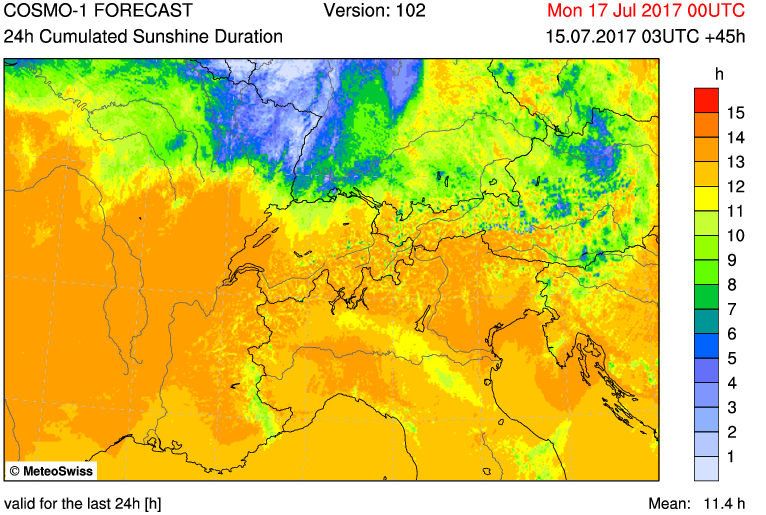
\includegraphics[width=\hsize]{klima/cosmo1.png}
\caption{COSMO-1 24-Stunden-Summe Vorhersage für Sonnenschein \cite{klima:meteoschweiz}
\label{klima:wettervorhersagen:cosmo}}
\end{figure}

\begin{itemize}
\item COSMO-1: 1158 x 774 Gitterpunkte; Maschenweite 1.1 km (0°01'); 80 vertikale Schichten; gesamter Alpenbogen mit der Schweiz im Zentrum; Zeitschrittweite 10 Sekunden; Voraussagen bis 45h, 8mal täglich; Geeignet für bessere Vorhersagen, insbesondere Gewitter, thermische Windsysteme und Föhn \cite{klima:meteoschweiz}
% Funfact, CFL = 10s / 1100m * 343 m/s = 3.12 Es scheint das Wettervorhersagen mit COSMO bereits bei einer Courant-Friedrich-Levi-Zahl von ca. 3.12 verlässlich sind. Üblich ist in numerischen Simulationen ein Wert von 1, dies würde jedoch einen 3mal höheren Rechenaufwand bedeuten.
\item COSMO-7: 393 x 338 Gitterpunkte; Maschenweite 6.6 km (0° 06'); 60 vertikale Schichten; ganz West- und Mitteleuropa; Voraussagen bis 72h, 3mal täglich \cite{klima:meteoschweiz} 
\item COSMO-E: 582 x 390 Gitterpunkte; Maschenweite 2.2 km (0° 02'); 60 vertikale Schichten; gesamter Alpenbogen mit der Schweiz im Zentrum; 21 Ensemble-Rechnungen mit leicht variierenden Initialwerten mit gleich wahrscheinlichen Vorhersagen; Geeignet für Wahrscheinlichkeitsvorhersagen von extremen Ereignissen wie Stürme oder Starkniederschläge \cite{klima:meteoschweiz} 
\end{itemize}


\subsection{Klimavorhersagen
\label{subsection:klima:entstehung}}
\rhead{Klimavorhersagen}
Die Weltorganisation für Meteorologie (WMO) definiert das Klima als die Statistik des Wetters über einen Zeitraum, der lang genug ist, um diese statistischen Eigenschaften auch bestimmen zu können. Während das Wetter den physikalischen Zustand der Atmosphäre zu einem bestimmten Zeitpunkt an einem bestimmten Ort beschreibt, ist Klima erst dann richtig gekennzeichnet, wenn die Wahrscheinlichkeit für Abweichungen vom Mittelwert angegeben werden kann, also auch Extremwerte Teil der Statistik sind. Zur Beschreibung des Klimas wird in der Regel eine Zeitspanne von 30 Jahren als Bezugszeitraum herangezogen. Die übliche Einteilung in Klimazonen folgt überwiegend dem Jahresgang der Temperatur und des Niederschlags. \cite{klima:maxplanck}

Die ersten Klimamodellen wurden bereits in den 1960er Jahren genutzt, es handelte sich im wesentlichen um einfache Energiebilanzmodelle von Strahlung und Wärme. Eine Modellierung der Atmosphäre wäre zu dieser Zeit aufgrund der fehlenden Rechenkapazität nicht möglich gewesen. Jedoch konnten auch mit diesen einfachen Modellen bereits Aussagen zum Temperaturanstieg aufgrund des $CO_2$ anstiegs getätigt werden. In den 1970er Jahren wurden, wegen der steigenden Rechenkapazität, erstmals Wettervorhersagemodelle für die Klimaforschung eingesetzt. Dies bringt einige Vorteile mit sich, so müssen keine Programme von Grund auf neu entwickelt werden. Ein Nachteil liegt jedoch in den grossen Rechenleistungen welche, wie beim Wetter, für zuverlässige Aussagen benötigt werden.
 
Es gibt viele verschiedene Parameter welche einen Einfluss auf das Klima haben, so gehören dazu  allgemeine Dinge wie Sonneneinstrahlung, zusammensetzung der Atmosphäre und Oberflächenbeschaffenheit (Wasser, Wüste, Wälder, Wiese, etc.). Seit der industriallisierung beinflusst der Mensch die Luftzusammensetzung mit dem vermehrten Ausstoss von $CO_2$, jedoch ist dies nicht die einzige Einflussnahme des Menschen, so gibt es viele Dinge welche sich direkt oder indirekt auf das Klima auswirken. Als Beispiel setzt die Abholzungen von Wäldern zusätzlich $CO_2$ frei. Wälder sind jedoch auch hervorragende Wasserspeicher, dieses Wasser verdunstet und ist oft für Regen in trockeneren Gebieten verantwortlich. Sind die Wälder nicht mehr vorhanden können andere Regionen plötzlich mit Trockenheit zu kämpfen haben.

Das Klima ist ein heickles System, so weist es verschiedenste Kipppunkte und Rückkopplungseffekte auf. So beschreibt die Eis-Albedo-Rückkopplung den Effekt der Rückstrahlung der Sonnenstrahlen auf Eis, wie zum Beispiel in der Arktis. Sollte dieses Eis verschwinden und dafür das arktische Meer die Oberfläche bilden wird die Sonnenstrahlung zu einem grossenteil absorbiert und nicht mehr zurück in den Weltraum gestrahlt. Hierbei wandelt sich die Strahlung in Wärme um und sorgt für eine noch schnellere erwärmung unseres Klimasystems. Eine weitere Rückkopplung bildet Methan, ebenfalls ein Treibhausgas, welches in den Permafrostböden von Kanada und Russland liegt, welches durch das auftauen dieser in die Atmosphäre gelangt. Es gibt auch unscheinbare Rückkopplungen, so gelingt durch die Klimaerwärmung zusätzlich Wasserdampf, ein natürliches Treibhausgas, in die Atmosphäre und sorgt für eine weitere Erwärmung des Klimasystems.


\section{Spektrale Methoden
\label{section:klima:spektrale}}
\rhead{Beispiel}
Im Gegensatz zur klassischen Strömungsmechanik, welche mit Differenzmethoden arbeiten, wählen die Spektralen Methoden einen globalen Ansatz. Hierbei wird das Ergebniss in den Spektralbereich bereich transformiert und ist keine physikalische grösse wie Druck oder Temperatur. Als effizientes Verfahren zur Hin- und Rücktransformation der Spektral-Koeffizienten bietet sich die schnelle Fouriertransformation (FFT) an, auf diese wird hier jedoch nicht eingegangen.


\subsection{Beispiel Wärmeleitungsgleichung}
Wie im vorherigen Kapitel \ref{subsection:klima:entstehung} \nameref{subsection:klima:entstehung} aufgezeigt handelt es sich bei unserer Atmosphäre um ein hochkomplexes System deren Eigenheiten bis zum heutigen Zeitpunkt noch nicht restlos verstanden sind und deshalb immer noch Teil der Forschung ist. Ein komplexes System wie das Klima kann somit unmöglich in einigen wenigen Zeilen mathematisch hergeleitet und beschrieben werden. Wir schränken uns aus diesem Grund bei den Beispielen auf ein einziges Problem, die Wärmeleitung, ein. Die Problemstellung ist einfach zu verstehen, veranschaulicht jedoch die mathematischen Schwierigkeiten und deren komplexität sehr gut.

Für die Aufgaben wird die allgemeine Wärmeleitungsgleichung benötigt:
\begin{equation}
\frac{\partial T}{\partial t} =  \Delta T 
\label{klima:bsp:pdgl}
\end{equation}



\subsection{Lösung der Wärmeleitungsgleichung mit Differenzenmethoden}
Damit wir die komplexität eines herkömmlichen Modells, welches mit Differenzen arbeitet, mit dem der Spektralen Methoden vergleichen können, schauen wir dies an einem vereinfachten Beispiel an. Wir betrachten die Wärmeleitung eines Stabes.
Der Laplace-Operator ist bei einem eindimensionalen Problem gerade die zweite Ableitung selbiger, somit ergibt sich eine vereinfachte Wärmeleitungsgleichung.
\begin{equation}
\Delta T = \frac{\partial T}{\partial t}=\dfrac{\partial^2 T}{\partial x^2}
\end{equation}
Es werden die dazugehörigen Differenzenquotienten benötigt.
\begin{align}
\frac{\partial T}{\partial t}
&\rightarrow
\frac{\triangle T}{\triangle t}=
\frac{T(t+\triangle t,x)-T(t,x)}{\triangle t}
\\
\frac{\partial^2 T}{\partial x^2}
&\rightarrow
\frac{T(t,x+\triangle x)-2T(t,x)+T(t,x-\triangle x}{\triangle x^2}
\end{align}
Mit diesen lässt sich nun die Formel, welche für die numerische Berechnung benötigt wird, erstellen.
\begin{equation}
\frac{T(t+\triangle t,x)-T(t,x)}{\triangle t}
=
\frac{T(t,x+\triangle x)-2T(t,x)+T(t,x-\triangle x)}{\triangle x^2}
\label{klima:bsp:diff}
\end{equation}
\begin{figure}
\centering
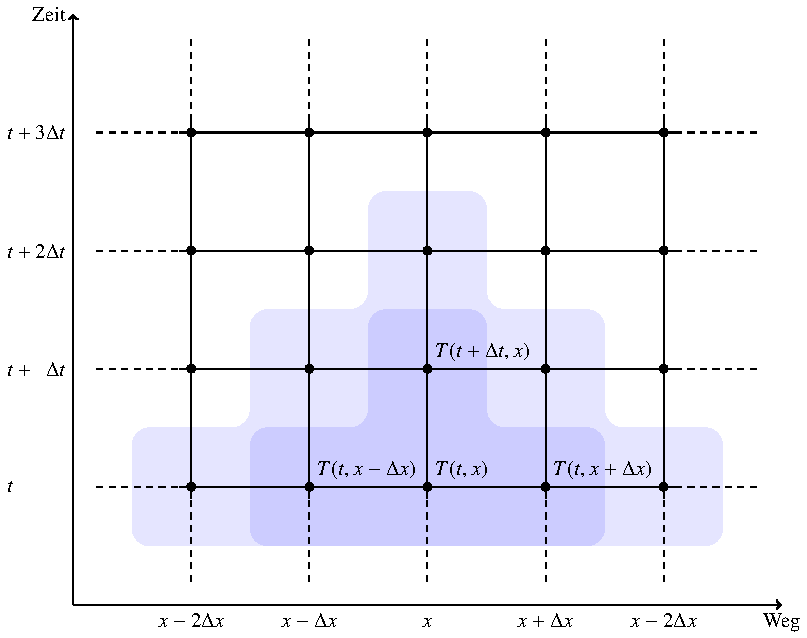
\includegraphics[width=\hsize]{klima/differenzen.pdf}
\caption{
\label{klima:wettervorhersagen:diff}}
\end{figure}
Mit der Gleichung \eqref{klima:bsp:diff} wird die Temperaturänderung bis zum nächsten Zeitschritt berechnet. Dies ist ebenso in der Abbildung~\ref{klima:wettervorhersagen:diff} illustriert. Wir können daher sagen, möchte man die Temperaturänderung eines Punktes zu seinem vorherigen Zustand wissen, so benötigt man die Werte der beiden benachbarten Punkte $x+\triangle x$ und $x-\triangle x$. Daraus lässt sich schlussfolgern dass sich Einflüsse in der Simulation maximal mit $\frac{\triangle x}{\triangle t}$ ausbreiten können. Sollte eine Problemstellung bearbeitet werden in welcher sich etwas schneller ausbreitet als dies in der Simulation geschehen kann führt dies zu Fehlern in der Auswertung. Möchte man das Problem angehen, so kann man die entweder die Punktabstände $\triangle x$ erhöhen oder den Zeitschritt $\triangle t$ verkleinern, dies führt jedoch zu erhöhtem Rechenaufwand. Es ist festzuhalten dass Modelle, welche auf den Differenzmethoden beruhen, eine endliche Ausbreitungungsgeschwindigkeit haben.

Möchte man mit den Differenzmethoden eine Simulation durchführen bedingt dies, dass diese Berechnungen für jeden Punkt zu jedem Zeitschritt gemacht werden muss. Dies führt dazu, dass Simulationen sehr Rechenintensiv sind.


\subsection{Lösung der Wärmeleitungsgleichung mit Spektralen Methoden}
Für die Spektralen Methoden werden im wesentlichen die Wärmeleitungsgleichung \eqref{klima:bsp:pdgl}
und eine Ansatzfunktion, wie die Fourier-Reihen, benötigt.


\subsubsection{Lösung der Wärmeleitungsgleichung}
Eine Übungsaufgabe, mit der Wärmeleitegleichung auf einem Kreis, befindet sich am Ende des Kapitels \ref{skript:chapter:kugelfunktionen} \nameref{skript:chapter:kugelfunktionen} auf der Seite \pageref{skript:1101:pdgl}.

Für die Konstruktion unseres Modells wird die Fourier-Reihe auf der Kugel benötigt:
\begin{equation}
T(\vartheta ,\varphi ,t)
=
a^0_0(t) + \sum_{l=1}^\infty\sum_{m=0}^l \bigl( a^m_l(t)Y^m_l(\vartheta ,\varphi)+b^m_l(t)Z^m_l(\vartheta ,\varphi)\bigr)
\label{equation:klima:fourier}
\end{equation}
Diese stellt im wesentlichen das Modell dar, $\vartheta$ steht dabei für den Längengrad und $\varphi$ für den Breitengrad. Zur berechnung der Koeffizienten $a^m_l(t)$ und $b^m_l(t)$ wird die folgende Form des Laplace-Operators benötigt:
\begin{equation}
\Delta Y^m_l=-l(l+1)Y^m_l
\label{equation:klima:laplace}
\end{equation}

Als erstes stellen wir die gewöhnliche Differentialgleichung auf, dazu muss die Fourier-Reihe~\eqref{equation:klima:fourier} für $T(\vartheta ,\varphi ,t)$ in die Differentialgleichung~\eqref{klima:bsp:pdgl} eingesetzt werden.
Dazu berechnen wir die Ableitungen nach $t$ und setzen die Gleichung \eqref{equation:klima:laplace} ein.
\begin{align*}
\frac{\partial T(\vartheta ,\varphi ,t)}{\partial t} &=
\dot{a}^0_0(t)+\sum_{l=1}^\infty\sum_{m=0}^l \bigl( \dot{a}^m_l(t)Y^m_l(\vartheta ,\varphi)+\dot{b}^m_l(t)Z^m_l(\vartheta ,\varphi)\bigr)
\\
\Delta T(\vartheta ,\varphi ,t) &=
- \sum_{l=1}^\infty\sum_{m=0}^l \bigl( a^m_l(t)l(l+1)Y^m_l(\vartheta ,\varphi)+b^m_l(t)l(l+1)Z^m_l(\vartheta ,\varphi)\bigr)
\end{align*}
Die Differentialgleichung verlangt, dass diese beiden Terme übereinstimmen, also folgen die gewöhnlichen Differentialgleichungen
\begin{align*}
\dot a^0_0(t)&= 0
\\
\dot a^m_l(t)&=l(l+1)a^m_l(t)&
\dot b^m_l(t)&=l(l+1)b^m_l(t)
\end{align*}
Man beachte, dass die erste Gleichung als Speziallfall in der ersten
Gleichung der zweiten Zeile enthalten ist.
\begin{align*}
a^0_0(t)&=const.
\\
a^m_l(t) &=Ae^{-l(l+1)t}&
b^m_l(t) &=Be^{-l(l+1)t}
\end{align*}

Möchte man die Kugelfunktionen $Y^m_l$ und $Z^m_l$ berechnen, so kann dies mit der Gleichung \eqref{skript:kugelfunktione:Y} auf der Seite \pageref{skript:kugelfunktione:Y} gemacht werden. Dies ist jedoch für das Verständniss nicht notwendig, so beschreiben diese Funktionen lediglich den Unterschied zum Mittelwert $a^0_0(t)$, in diesem Falle der globalen Mitteltemperatur. Wie sich der Unterschied entwickeln wird ist durch die $a^m_l(t)$ und $b^m_l(t)$ definiert.


\subsubsection{Konstanter Erwärmungsterm
\label{subsubsection:klima:erwaermungsterm}}
Wie wir im vorherigen Abschnitt gesehen haben ist die Lösung für die globale Mitteltempratur $a^0_0(t)=const.$, wenn dies wirklich so währe, gäbe es keine Klimaerwärmung. Da uns bekannt ist, dass diese exisstiert muss dies umgeschrieben werden.
\begin{equation}
a^0_0(t)=\phi^c(t)+ T_0
\end{equation}
$T_0$ stellt dabei, wie in den meisten Klimamodellen, die globale Temperatur vor der industriellen Zeit dar (ca. 1850). (Genauso verhält sich dies in der Abbildung~\ref{klima:einleitung:nasa}.) Das bedeutet dass der $CO_2$ anstieg bestandteil von $\phi^c$ sein muss. Dies könnte wie folgt aussehen 
\begin{equation}
\phi^c(t)=\delta_{CO2}+\delta_{Methan}+\delta_{Wasserdampf}+...
\end{equation}
Mit dem $\phi^c$ kann nun der Anstieg der globalen Mitteltemperatur berechnet werden.


\subsubsection{Temperaturunterschiede zwischen Nord- und Südhalbkugel
\label{subsubsection:klima:halbkugel}}
Möchte man ein kleines Klimamodell definieren, so muss  $m$ und $l$ festgelegt werden, diese ist Abhängig von der Komplexität welche erreicht werden möchte. Da wir in unserem Beispiel diese klein halten wollen entscheiden wir uns für $l=1$ und $m=0$, dieses Beispiel gliedert unseren Planeten in der Modellierung in Nord- und Südhalbkugel auf. Mit höheren $m$ und $l$ würden wir unseren Planeten in weitere Bereiche gliedern und die Modellierung komplexer gestalten, jedoch möchten wir genau dies nicht.
\begin{align*}
a^0_0(t)&=\phi^c(t)+T_0
\\
a^0_1(t) &=Ae^{-2t}&
b^0_1(t) &=Be^{-2t}
\end{align*}
Aus der Gleichung \eqref{equation:klima:fourier} entsteht folgende:
\begin{align}
T(\vartheta ,\varphi ,t)
=
\underbrace{a^0_0(t)}_{Global} + \underbrace{a^0_1(t)Y^0_1(\vartheta ,\varphi)}_{Nordhalbkugel}+\underbrace{b^0_1(t)Z^0_1(\vartheta ,\varphi)}_{S"udhalbkugel} 
\end{align}
Ein Grossteil der $CO_2$ Emissionen, ein Treibhausgas, geschehen auf der Nordhalbkugel. Dies hat einen direkten Einfluss darauf, dass sich das Klima auf der Nordhalbkugel wegen der grösseren $CO_2$ konzentrationen mehr erwärmt, dies führt zu einem Rückkopplungseffekt. Somit muss die Funktion $\dot a_0^1(t)$ folgendermassen modifiziert werden, das $\delta_{CO2}(t)$ stellt dabei die zusätzliche Erwärmung dar.
\begin{align*}
\dot a_0^1(t) &= 2a_1^0+\delta_{CO2} &
a_1^0 &= Ae^{-2t-\delta_{CO2}(t)}
\end{align*}
Ebenso kann man die unterschiedlichen Einflüsse der Jahreszeiten modellieren. So ist die Sonneneinstrahlung unteranderem von der Jahreszeit abhängig, dies könnte in der Modellierung folgendermassen ausschauen:
\begin{align*}
\dot a_1^0(t) &= 2a_1^0 \cos(\theta_{Jahr}(t)) &
\dot b_1^0(t) &= 2a_1^0 \sin(\theta_{Jahr}(t))
\\
a_1^0 &= Ae^{-2t \cos(\theta_{Jahr}(t)} &
b_1^0 &= Be^{-2t \sin(\theta_{Jahr}(t)}
\end{align*}


\subsection{Anwendung der spektralen Methoden}
In den vorherigen Abschnitten wurden Beispiele für die Differenzenmethode und die spektralen Methoden anhand der Wärmleitungsgleichung gezeigt. Dabei lassen sich bereits wesentlich Vorteile der spektralen Methoden erkennen, so ist diese nicht auf Zeitschritte angewiesen, beschreiben nicht nur einzelne Punkte sondern ganze Gebiete und zusätzliche Einflussfaktoren können relativ einfach hineinmodelliert werden.
 
Die Spektralen Methoden werden heute bereits in einigen Modellen eingesetzt, so beispielsweise beim \textit{Integrated Forecast System} (IFS) einem globalen Wettervorhersage-Modell des \textit{Europäischen Zentrums für mittelfristige Wettervorhersagen}(ECWMF). So wurde dort bereits im April 1983 das erste spektrale Modell in Betrieb genommen.\cite{klima:ecmwf}


\printbibliography[heading=subbibliography]
\end{refsection}